\documentclass[11pt]{article}

% ---------------- Packages ----------------
\usepackage[margin=1in]{geometry}
\usepackage{amsmath,amssymb,amsthm}
\usepackage{graphicx}
\usepackage{hyperref}
\usepackage{fancyhdr}
\usepackage{enumitem}
\usepackage[UTF8]{ctex}
\usepackage{algorithm}
\usepackage{algpseudocode}
% ---------------- Header ----------------
\pagestyle{fancy}
\fancyhf{}
\lhead{Course Name}
\rhead{Homework \#1}
\cfoot{\thepage}

% ---------------- Title ----------------
\title{Homework 1}
\author{羊瑞 \\ 2300013091}
\date{\today}

% ---------------- Custom commands ----------------
\newcommand{\R}{\mathbb{R}}
\newcommand{\E}{\mathbb{E}}

% ---------------- Problem Environment ----------------
\newcounter{problem}

\newenvironment{problem}[1][]{
\stepcounter{problem}
\section*{Problem \theproblem\; #1}
}{}

\newenvironment{solution}{
\par\noindent\textbf{Solution.}\par\noindent
}{\qed}

\setlength{\parindent}{0pt}
% ---------------- Document ----------------
\begin{document}

\maketitle

\begin{problem} 
\begin{center}
    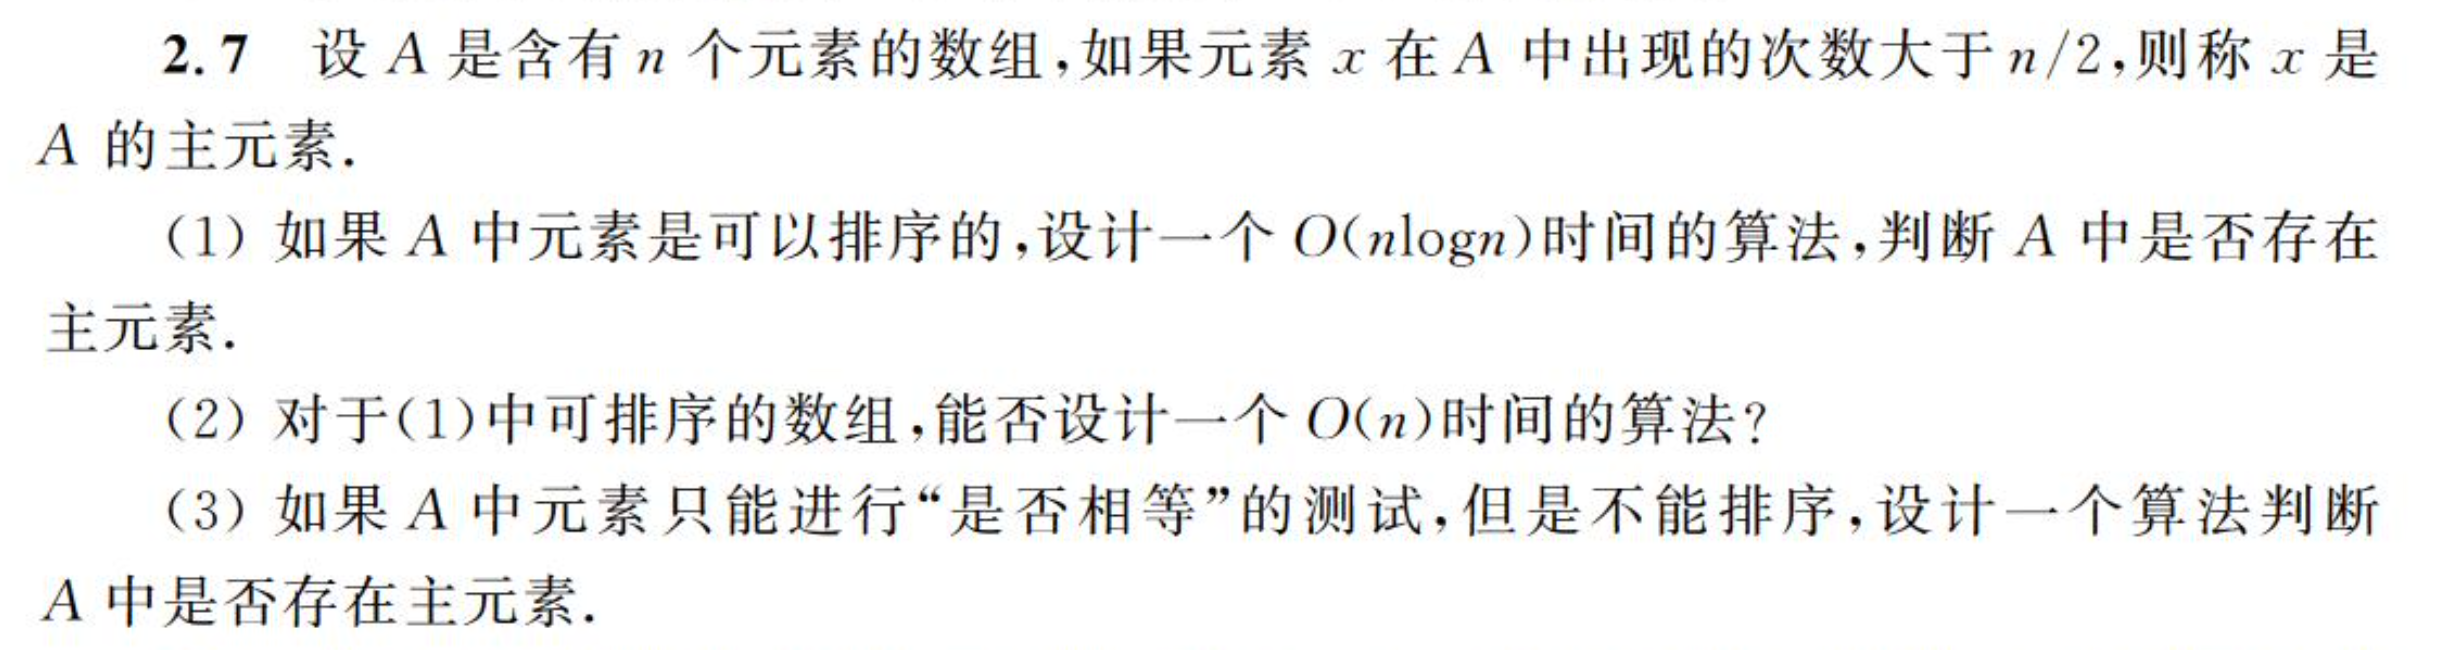
\includegraphics[width=0.6\textwidth]{problems/2-7.png}
\end{center}
\end{problem}

\begin{solution}
(1) 首先使用快速排序的方法对A中元素进行排序, 这一步的时间复杂度为 $O(nlogn)$. 设x为A中出现次数最多的元素, 初始化x=A[0], 对x对出现次数遍历计数. 当新元素和x不相等时, 比较x的出现次数是否是当前最大的，如果是则替换x, 并对元素接着计数, 这一步的复杂度为 $O(n)$. 最后若x的出现次数大于n/2, 那么x为A的主元素, 否则A没有主元素. 总的算法复杂度为 $T(n) = O(nlogn) + O(n) = O(nlogn) $. \\
(2) 主元素一定是数组的中位数, 否则中位数一侧有少于n/2-1个数, 这与中位数的定义矛盾. 找到中位数只需要O(n)复杂度， 接着统计中位数在数组中出现的次数, 也是O(n), $T(n) = O(n) + O(n) = O(n) $. \\
(3) 取一个大小为$\lceil \frac{n}{2} \rceil$的栈, 依次取A中元素, 然后若栈为空, 将x入栈, 否则将x与栈顶元素比较“是否相等”, 若不然则两个元素均出栈, 相等则将x入栈. 最后栈中如果有剩余的元素, 那么其就是主元素, 若栈为空则数组没有主元素. 正确性: 每次操作结束后, 栈中元素均相等, 否则有两个相邻元素不相等, 这与操作规则矛盾. 最后结束时, 若有剩余元素且不是主元素, 主元素出栈大于n/2次, 需要大于n/2个其他元素同时出栈, 元素数量不够, 矛盾.
\end{solution}

\begin{problem}
\begin{center}
    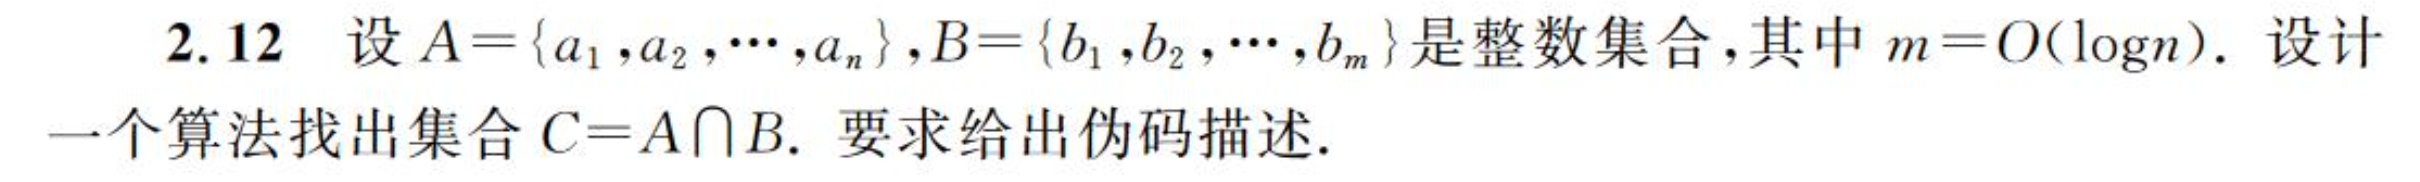
\includegraphics[width=0.6\textwidth]{problems/2-12.png}
\end{center}
\end{problem}

\begin{solution}
先对B进行排序, 再将A中各个元素在B中进行二分查找. \\
\begin{algorithmic}[1]
\State Input: A, B 
\State Output: $C = A \cap B$ \\
$C = \emptyset $ \\
$B' = QuickSort(B) $ 
\For{$i = 1$ to $n$}
    \State $x \leftarrow A[i]$
    \State $j \leftarrow BinarySearch(B', x)$
    \If{j > 0}
        \State $C \leftarrow C \cup$ {x}
    \EndIf
\EndFor

\end{algorithmic}

B的排序复杂度为 $O(mlogm)$, A中每个元素在B'中进行二分查找复杂度为 $O(logm)$, 总复杂度 $O(nlogm)$. $T(n) = O(mlogm) + O(nlogm) = O(nlogm) = O(nloglogn) $.
\end{solution}

\begin{problem}
\begin{center}
    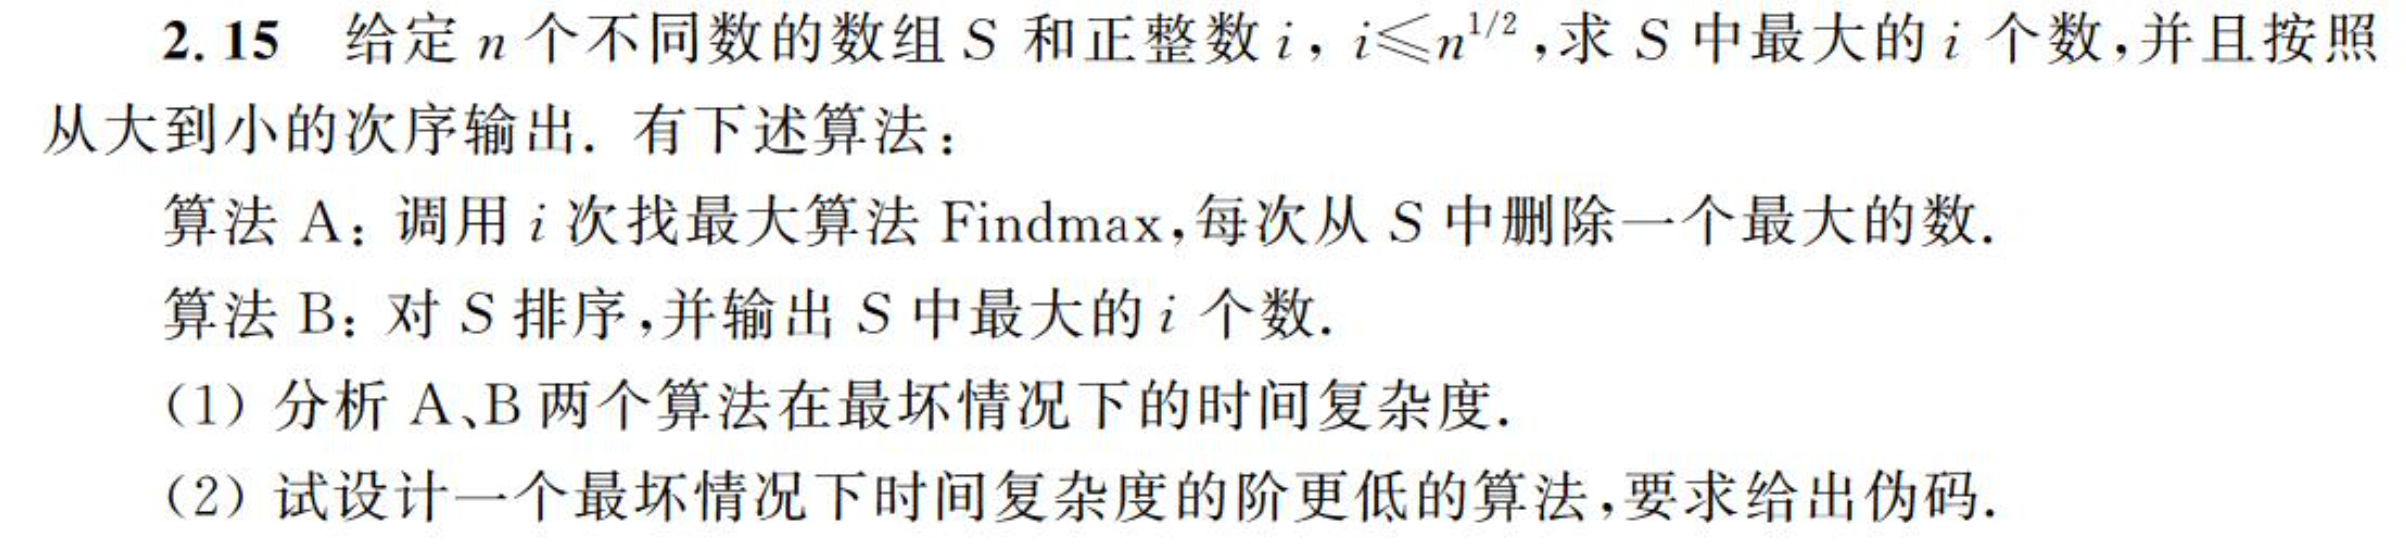
\includegraphics[width=0.6\textwidth]{problems/2-15.png}
\end{center}
\end{problem}

\begin{solution}
(1) A: $W(n) = O(in) = O(n^{3/2}) $ B: $O(nlogn) $ \\
(2) 
\begin{algorithmic}[1]
\State $k \leftarrow n-i+1 $ 
\State $x \leftarrow Select(S, k)$ 
\State $A[1..i] \leftarrow S$中不大于x的数 
\State 对A排序
\State 顺序输出A

\end{algorithmic}

时间复杂度 $T(n) = O(n) + O(\sqrt{n}log \sqrt{n}) = O(n)$.
\end{solution}

\begin{problem}
\begin{center}
    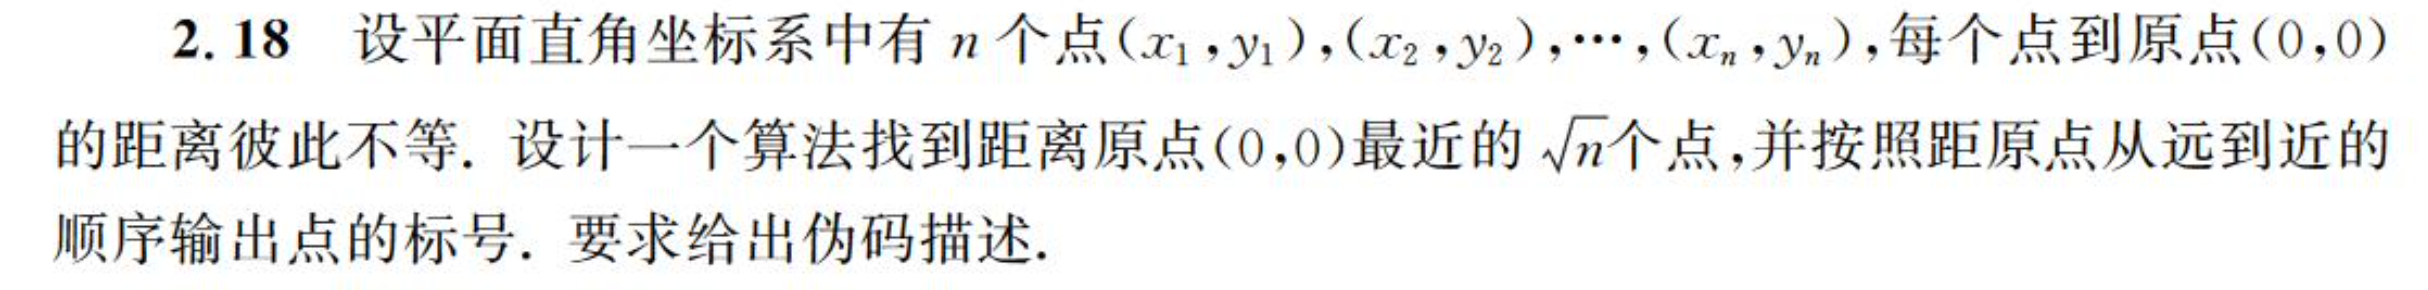
\includegraphics[width=0.6\textwidth]{problems/2-18.png}
\end{center}
\end{problem}

\begin{solution}
\begin{algorithmic}[1]
\State Input: $(x_1, y1), ..., (x_n, y_n)$
\State Output: 距离远点最近的$\sqrt{n}$个点的下标
\For{$i = 1$ to $n$}
    \State $d_i = \sqrt{x_i^2+y_i^2}$
    \State $d \leftarrow Select([d_1, ..., d_n], \sqrt{n})$
    \State 遍历距离数组, 若小于等于d, 则加入数组A并记录原下标
    \State 对A排序并顺序输出原下标
\EndFor

\end{algorithmic}

$T(n) = O(n) + O(\sqrt{n}log\sqrt{n}) = O(n) $
\end{solution}

\begin{problem}
\begin{center}
    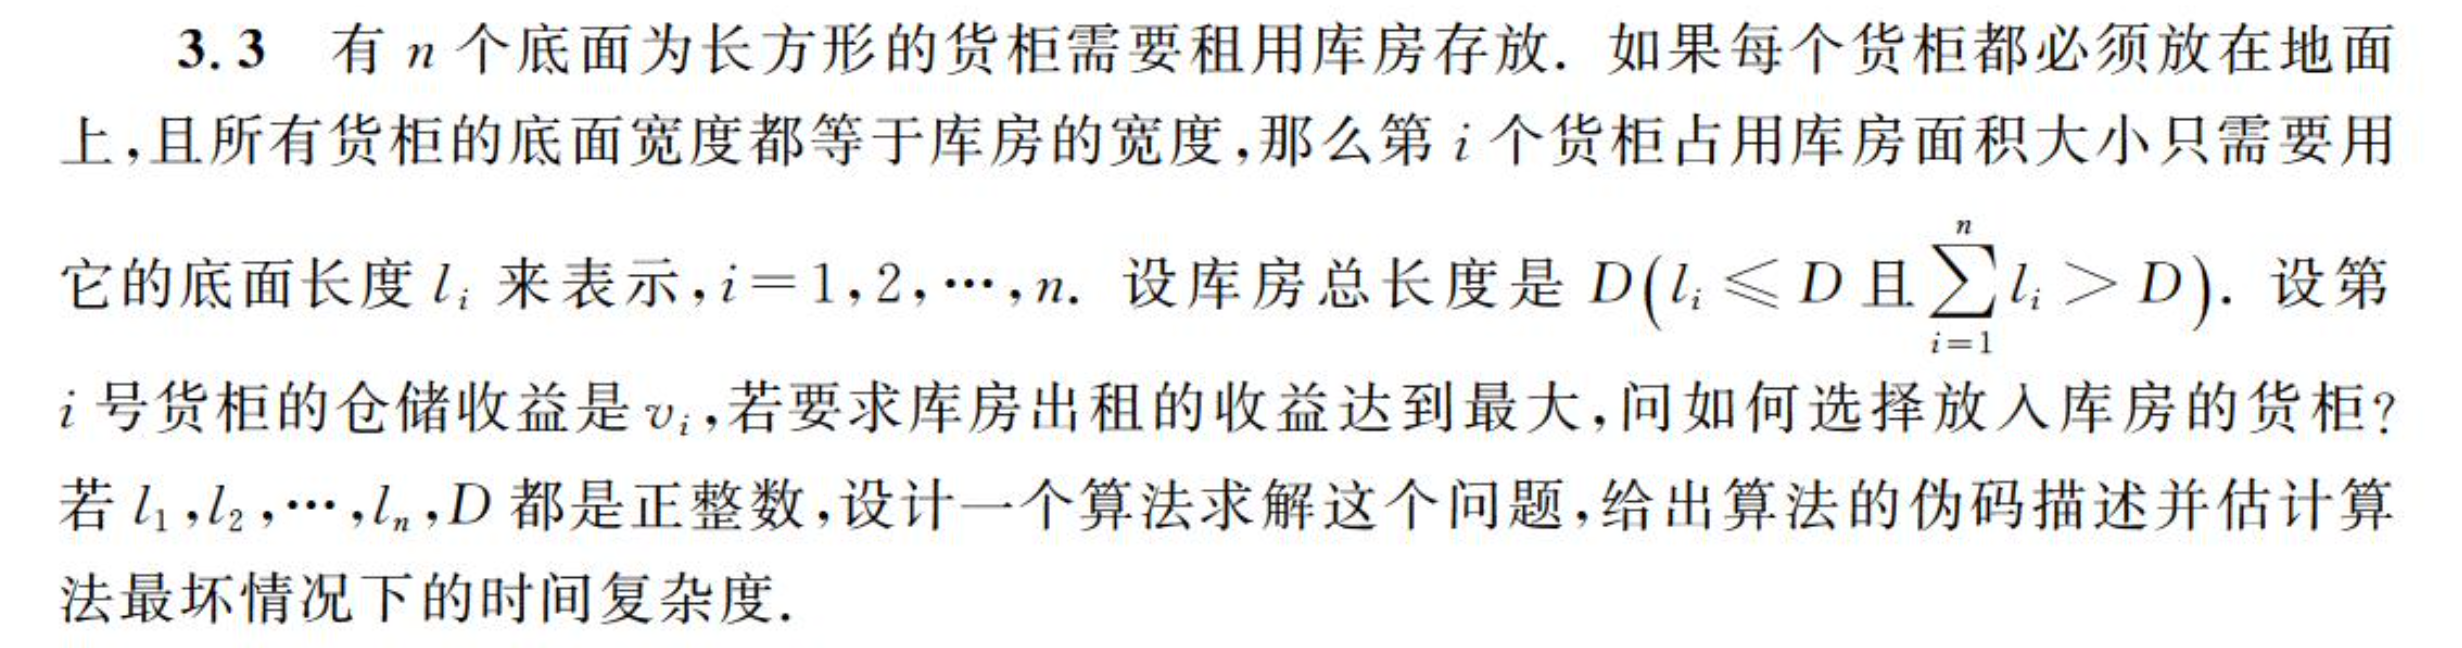
\includegraphics[width=0.6\textwidth]{problems/3-3.png}
\end{center}
\end{problem}

\begin{solution}

\begin{algorithmic}[1]

\State: Input:  $l_1, l_2, \dots, l_n$, $v_1, v_2, \dots, v_n$, $D$
\State: Output: 最大价值

\State Let $dp[0 \dots n][0 \dots D]$ be a 2D array

\For{$w = 0$ to $D$}
    \State $dp[0][w] \gets 0$
\EndFor

\For{$i = 1$ to $n$}
    \State $dp[i][0] \gets 0$
\EndFor

\For{$i = 1$ to $n$}
    \For{$w = 1$ to $D$}
        \If{$l_i > w$}
            \State $dp[i][w] \gets dp[i-1][w]$
        \Else
            \State $dp[i][w] \gets \max\{dp[i-1][w],\ dp[i-1][w-l_i] + v_i\}$
        \EndIf
    \EndFor
\EndFor

\State \Return $dp[n][D]$

\end{algorithmic}

复杂度O(nD).
\end{solution}

\begin{problem}
\begin{center}
    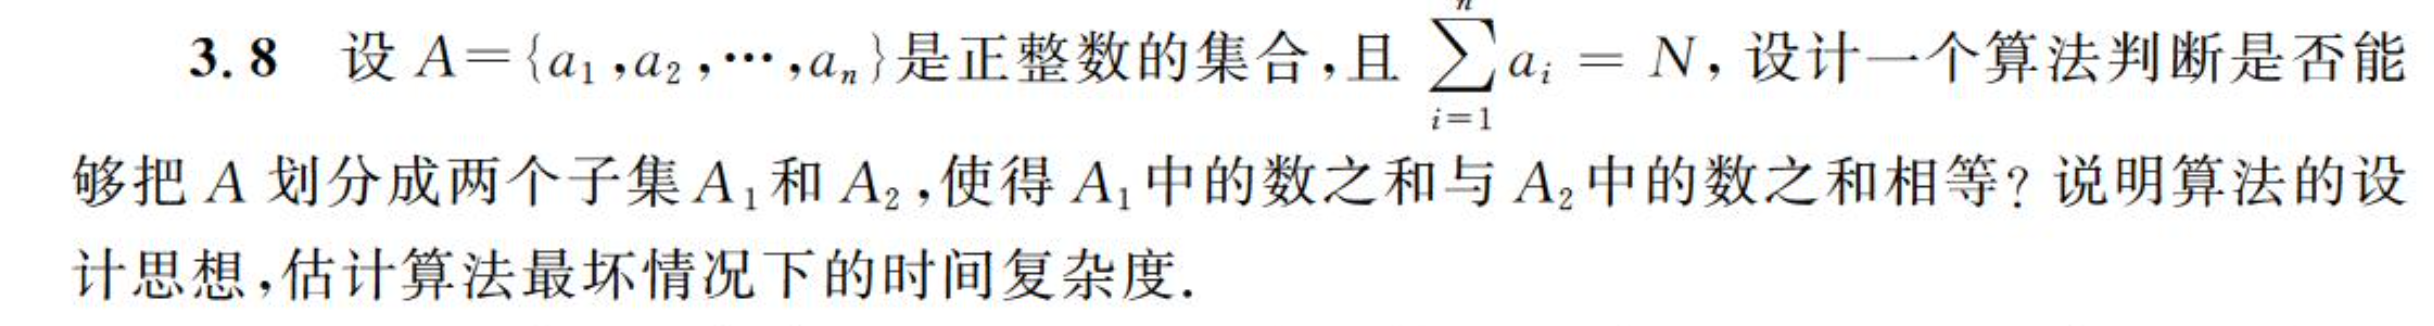
\includegraphics[width=0.6\textwidth]{problems/3-8.png}
\end{center}
\end{problem}

\begin{solution}
思想: 找到A是否存在子集 $A_1$, 使得其元素和为N/2, 用 $dp[i][j] $表示前i个数能否取出若干个使得和为j, 1表示可以, 0表示不行. 转移方程为: $dp[i][j] = dp[i-1][j] \lor dp[i-1][j-a_i] $, 最后检查dp[n][N/2].
\end{solution}

\begin{problem}
\begin{center}
    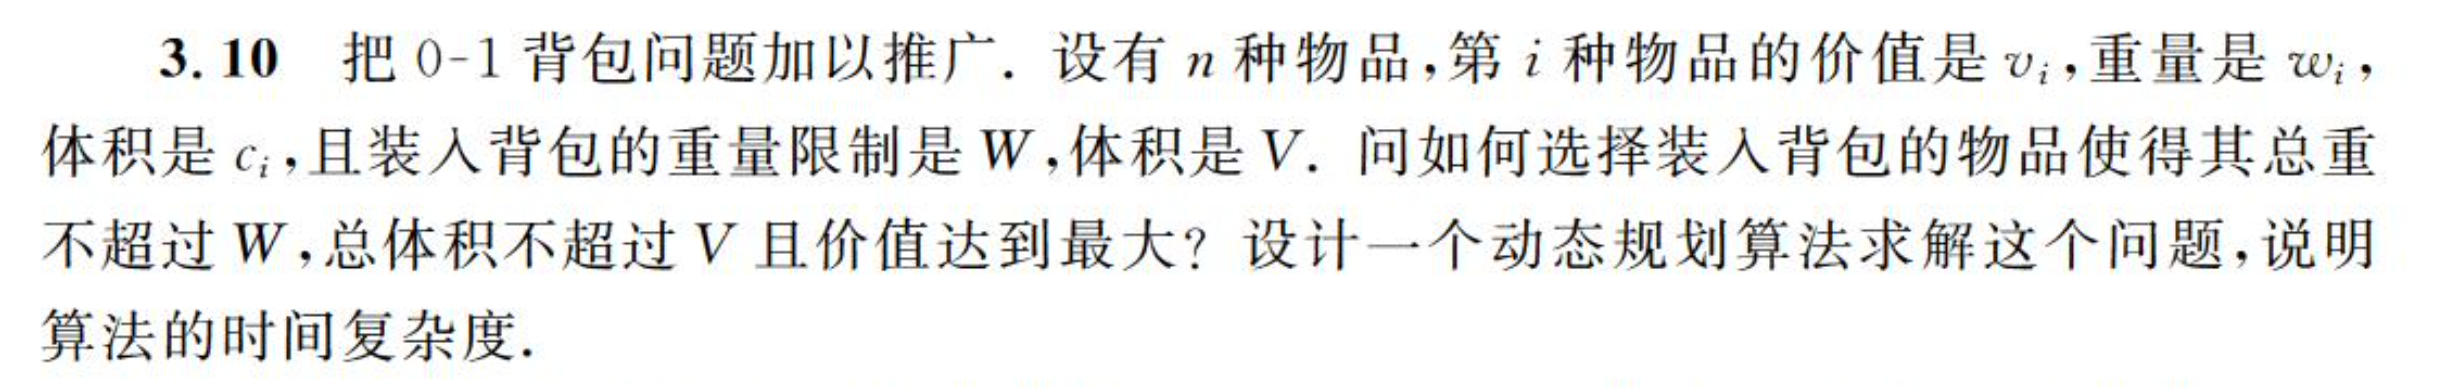
\includegraphics[width=0.6\textwidth]{problems/3-10.png}
\end{center}
\end{problem}

\begin{solution}
用 $dp[i][v][w] $表示从前i个物品中选择, 重量不超过w, 体积不超过v时能获得的最大价值. 初始化dp[i][v][w] = 0, 递推方程为 $dp[i][v][w] = max(dp[i-1][v][w], dp[i-1][v-c_i][w-w_i]+v_i) $. 最终能获得的最大价值为dp[n][V][W].
\end{solution}

\begin{problem}
\begin{center}
    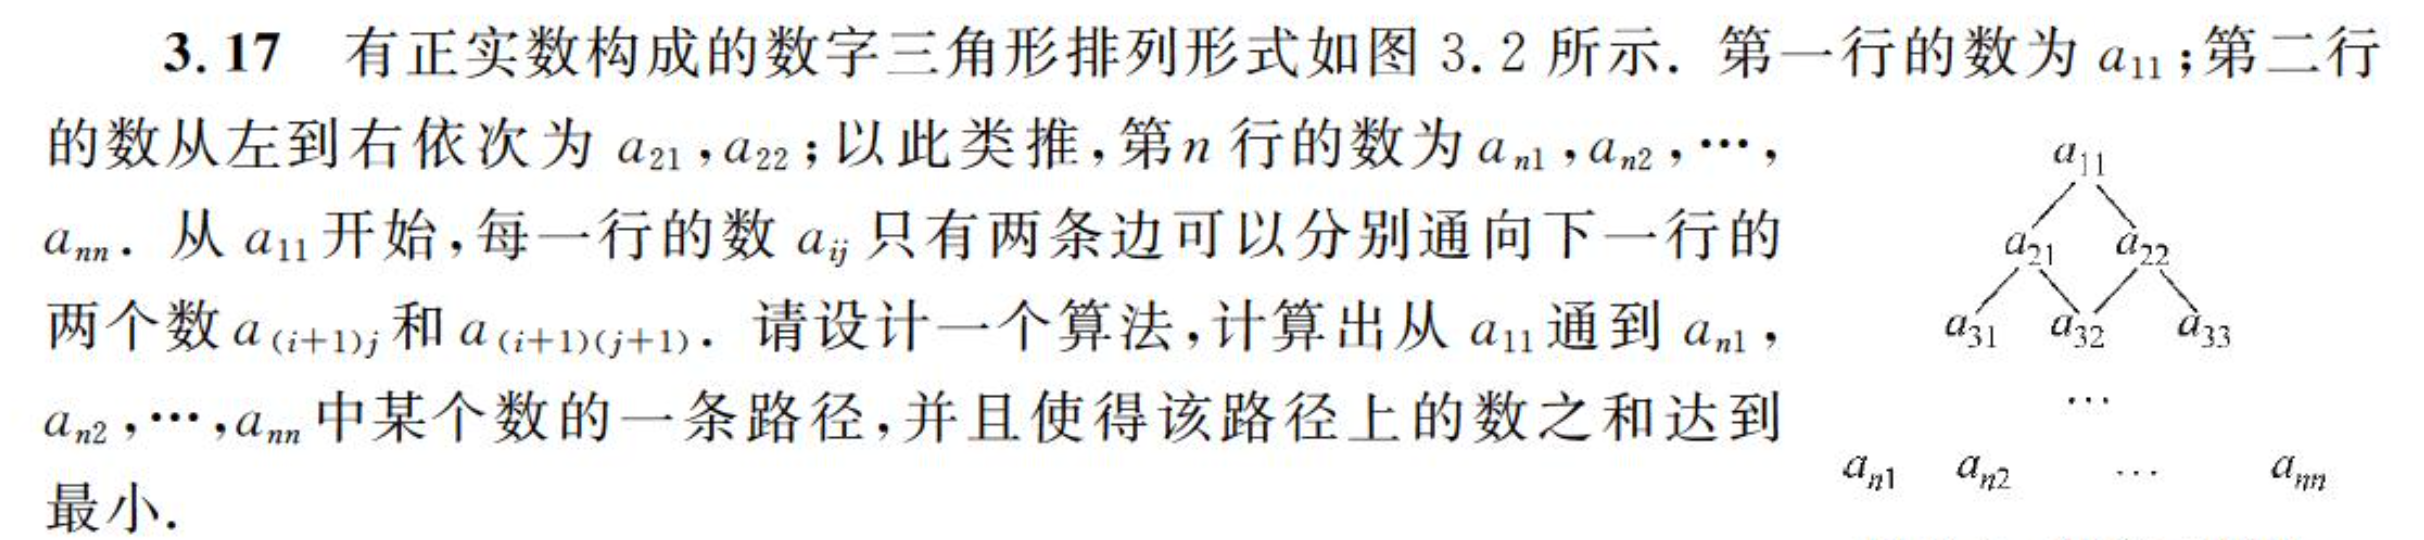
\includegraphics[width=0.6\textwidth]{problems/3-17.png}
\end{center}
\end{problem}

\begin{solution}
设 $dp[i][j] $是从$a_{11}$ 到 $a_{ij}$的所有路径中路径上数之和最小的值, 递推公式为 $dp[i][j] = a_{ij} + min(dp[i-1][j], dp[i-1][j-1]) $, 其中 $dp[i][0] = \infty, dp[i][i+1] = \infty $. 最后, 取 $max(dp[n][1], \dots, dp[n][n]) $, 即得到路径和最小值. 要求最小和路径, 只需额外维护一个前序数组, 按照递推公式选择哪一项选择对应的前驱.
\end{solution}

\end{document}